\documentclass[a4paper,11pt]{article}

\usepackage[utf8]{inputenc}

\usepackage{graphicx}
\usepackage{caption}
\usepackage{subcaption}

\usepackage{pgfplots}
\usepackage{float}
\usepackage{hyperref}
\usepackage{soul}
\hypersetup{
    colorlinks=true, % Enable colored links
    linkcolor=black, % Color for internal links
    urlcolor=black,  % Color for external links
    citecolor=black, % Color for citation links
    pdfborder={0 0 0}, % Remove border around links
}
\newcommand{\underlinehref}[2]{%
    \href{#1}{\ul{#2}}%
}
\pgfplotsset{compat=1.18}


\usepackage{minted}

\begin{document}

    \title{
        \textbf{Searching in arrays in C}
    }
    \author{Péter Herczku}
    \date{Fall 2024}

    \maketitle

    \section*{Introduction}
    \begin{figure}[h]
        \centering
        \begin{subfigure}[b]{.5\textwidth}
            \centering
            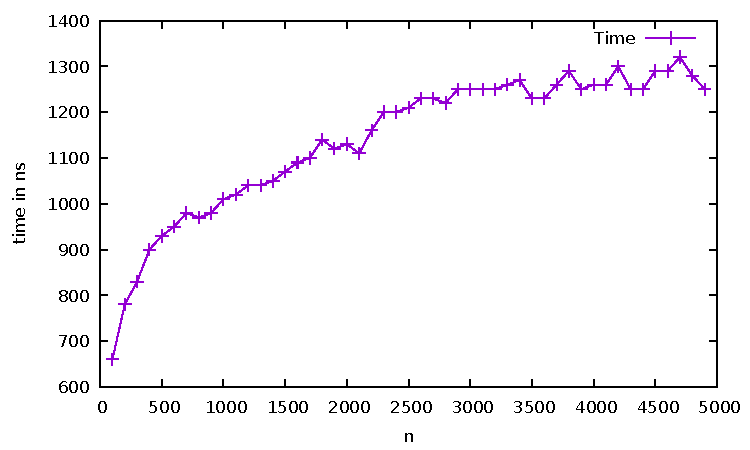
\includegraphics[width=\textwidth]{./binary_recursive/data} % Adjust width or height as needed
        \end{subfigure}
        \caption{Graph of binaryrecursive}
        \label{fig:graph_1}
    \end{figure}
    \begin{figure}[h]
        \centering
        \begin{subfigure}[b]{.5\textwidth}
            \centering
            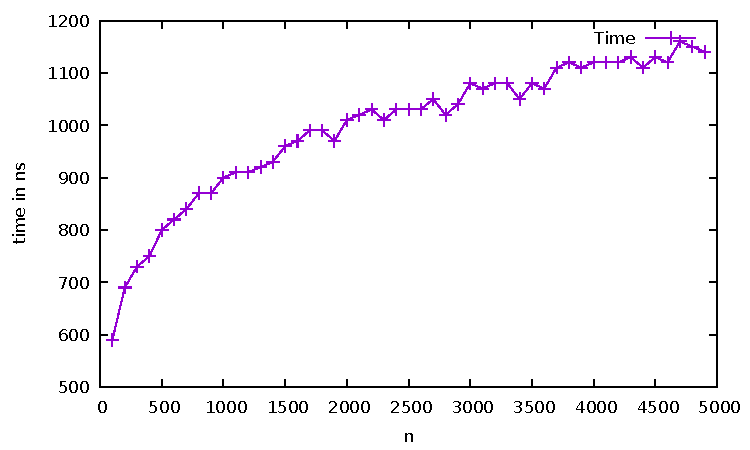
\includegraphics[width=\textwidth]{./binary_search/data} % Adjust width or height as needed
        \end{subfigure}
        \caption{Graph of binarysearch}
        \label{fig:graph_2}
    \end{figure}
    \begin{figure}[h]
        \centering
        \begin{subfigure}[b]{.5\textwidth}
            \centering
            \includegraphics[width=\textwidth]{./linear_sorted_with_optimization/data} % Adjust width or height as needed
        \end{subfigure}
        \caption{Graph of linearsortedwithoptimization}
        \label{fig:graph_3}
    \end{figure}
    \begin{figure}[h]
        \centering
        \begin{subfigure}[b]{.5\textwidth}
            \centering
            \includegraphics[width=\textwidth]{./unsorted/data} % Adjust width or height as needed
        \end{subfigure}
        \caption{Graph of unsorted}
        \label{fig:graph_4}
    \end{figure}

\end{document}
